\hypertarget{development-of-the-nervous-system-1}{%
\chapter{Development Of The Nervous System}\label{development-of-the-nervous-system-1}}

The development of the nervous system, or neural development, or neurodevelopment, refers to the processes that generate, shape, and reshape the nervous system of animals, from the earliest stages of embryonic development to adulthood. The field of neural development draws on both neuroscience and developmental biology to describe and provide insight into the cellular and molecular mechanisms by which complex nervous systems develop, from nematodes and fruit flies to mammals. Defects in neural development can lead to malformations and a wide variety of sensory, motor, and cognitive impairments neurological disorders and intellectual disability.

The central nervous system (CNS) is derived from the ectoderm---the outermost tissue layer of the embryo. In the third week of human embryonic development the neuroectoderm appears and forms the neural plate along the dorsal side of the embryo. The neural plate is the source of the majority of neurons and glial cells of the CNS. A groove forms along the long axis of the neural plate and, by week four of development, the neural plate wraps in on itself to give rise to the neural tube, which is filled with cerebrospinal fluid (CSF).

As the embryo develops, the anterior part of the neural tube forms three primary brain vesicles, which become the primary anatomical regions of the brain: the forebrain (prosencephalon), midbrain (mesencephalon), and hindbrain (rhombencephalon). These simple, early vesicles enlarge and further divide into the five secondary brain vesicles -- the telencephalon (future cerebral cortex and basal ganglia), diencephalon (future thalamus and hypothalamus), mesencephalon (future colliculi), metencephalon (future pons and cerebellum), and myelencephalon (future medulla). The CSF-filled central chamber is continuous from the telencephalon to the spinal cord, and constitutes the developing ventricular system of the CNS. Because the neural tube gives rise to the brain and spinal cord any mutations at this stage in development can lead to fatal deformities like anencephaly or lifelong disabilities like spina bifida. During this time, the walls of the neural tube contain neural stem cells, which drive brain growth as they divide many times. Gradually some of the cells stop dividing and differentiate into neurons and glial cells, which are the main cellular components of the CNS. The newly generated neurons migrate to different parts of the developing brain to self-organize into different brain structures. Once the neurons have reached their regional positions, they extend axons and dendrites, which allow them to communicate with other neurons via synapses. Synaptic communication between neurons leads to the establishment of functional neural circuits that mediate sensory and motor processing, and underlie behavior.



\begin{figure}

{\centering 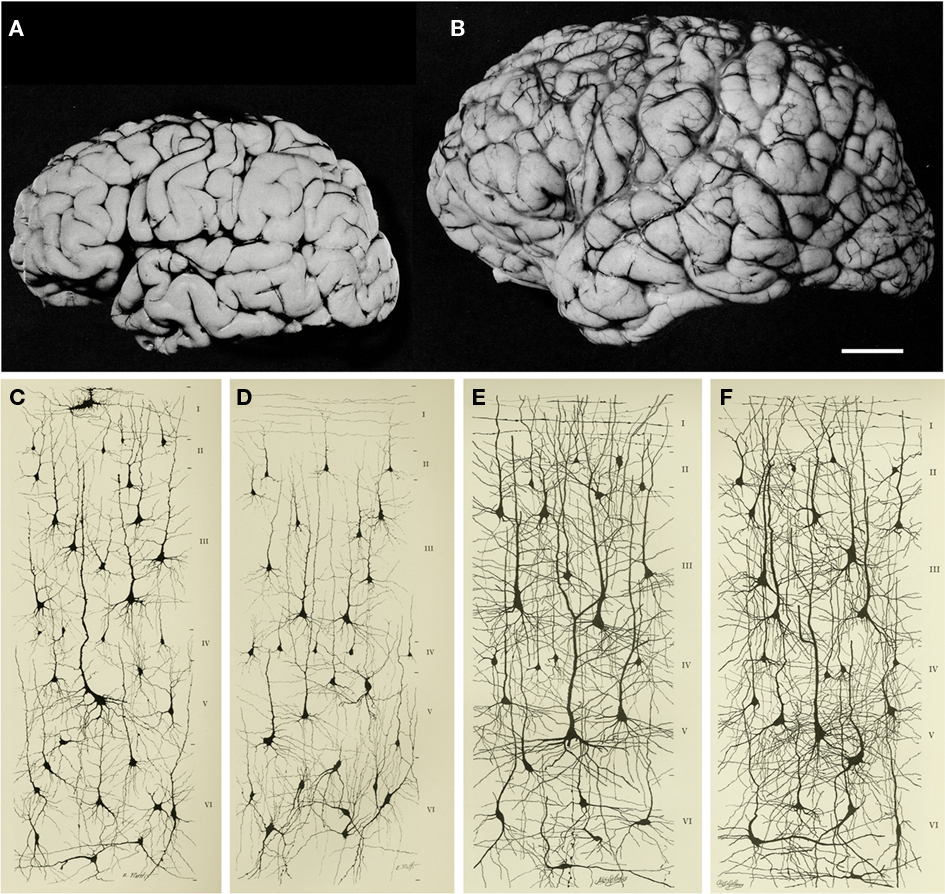
\includegraphics[width=0.7\linewidth]{./figures/development/fnana-05-00029-g004} 

}

\caption{Increase in brain size and the maturation of cortical circuits. The maturation of mental processes and motor skills is associated with an approximately fourfold enlargement in brain size. (A,B) photographs of the brains of a 1-month and 6-year-old-child. This increment is accompanied by a dramatic development in the complexity of the neuronal processes, which in turn is influenced by the genetic background and the environment. This increase in the complexity is clearly evident in the drawings of Golgi stained cortical neurons from the cerebral cortex of a 1-month {[}(C) ``pars triangularis of gyrus frontalis inferior''; (D) ``orbital gyrus''{]} and 6 year {[}(e), ``pars triangularis of gyrus frontalis inferior''; (F) ``orbital gyrus''{]} old child. Adapted from Conel and Le (1941, 1967). Scale bar for (A,B): 2 cm. From \href{https://www.frontiersin.org/article/10.3389/fnana.2011.00029}{DeFelipe J (2011) The evolution of the brain, the human nature of cortical circuits, and intellectual creativity. Front. Neuroanat. 5:29}}\label{fig:brainsize}
\end{figure}

\hypertarget{neural-induction}{%
\section{Neural Induction}\label{neural-induction}}

During early embryonic development the ectoderm becomes specified to give rise to the epidermis (skin) and the neural plate. The conversion of undifferentiated ectoderm to neuro-ectoderm requires signals from the mesoderm. At the onset of gastrulation presumptive mesodermal cells move through the dorsal blastopore lip and form a layer in between the endoderm and the ectoderm. These mesodermal cells that migrate along the dorsal midline give rise to a structure called the notochord. Ectodermal cells overlying the notochord develop into the neural plate in response to a diffusible signal produced by the notochord. The remainder of the ectoderm gives rise to the epidermis (skin). The ability of the mesoderm to convert the overlying ectoderm into neural tissue is called neural induction.

The neural plate folds outwards during the third week of gestation to form the neural groove. Beginning in the future neck region, the neural folds of this groove close to create the neural tube. The formation of the neural tube from the ectoderm is called neurulation. The ventral part of the neural tube is called the basal plate; the dorsal part is called the alar plate. The hollow interior is called the neural canal. By the end of the fourth week of gestation, the open ends of the neural tube, called the neuropores, close off.



\begin{figure}

{\centering 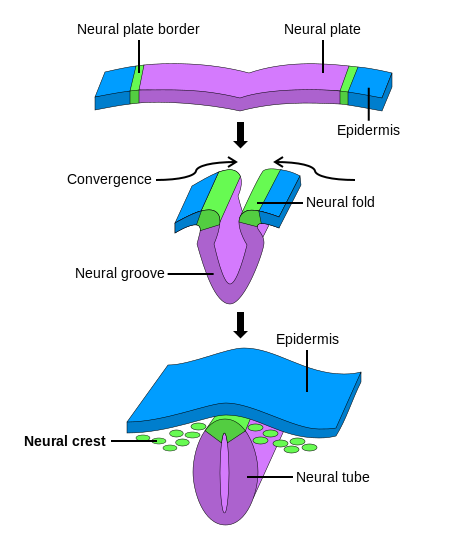
\includegraphics[width=0.7\linewidth]{./figures/development/neurulation} 

}

\caption{\href{https://en.wikipedia.org/wiki/Neural_tube\#/media/File:Neural_crest.svg}{A diagram of the stages of neural tube formation.}}\label{fig:neurulation}
\end{figure}

A transplanted blastopore lip can convert ectoderm into neural tissue and is said to have an inductive effect. Neural inducers are molecules that can induce the expression of neural genes in ectoderm explants without inducing mesodermal genes as well. Neural induction is often studied in \emph{Xenopus laevis} embryos since they have a simple body pattern and there are good markers to distinguish between neural and non-neural tissue. Examples of neural inducers are the molecules noggin and chordin.

When embryonic ectodermal cells are cultured at low density in the absence of mesodermal cells they undergo neural differentiation (express neural genes), suggesting that neural differentiation is the default fate of ectodermal cells. In explant cultures (which allow direct cell-cell interactions) the same cells differentiate into epidermis. This is due to the action of BMP4 (a TGF-β family protein) that induces ectodermal cultures to differentiate into epidermis. During neural induction, noggin and chordin are produced by the dorsal mesoderm (notochord) and diffuse into the overlying ectoderm to inhibit the activity of BMP4. This inhibition of BMP4 causes the cells to differentiate into neural cells. Inhibition of TGF-β and BMP (bone morphogenetic protein) signaling can efficiently induce neural tissue from human pluripotent stem cells, a model of early human development.

\hypertarget{the-early-brain}{%
\section{The Early Brain}\label{the-early-brain}}

Late in the fourth week, the superior part of the neural tube flexes at the level of the future midbrain---the mesencephalon. Above the mesencephalon is the prosencephalon (future forebrain) and beneath it is the rhombencephalon (future hindbrain). The optical vesicle (which will eventually become the optic nerve, retina and iris) forms at the basal plate of the prosencephalon.



\begin{figure}

{\centering \includegraphics[width=0.7\linewidth]{./figures/development/envhper00312-0143page3} 

}

\caption{Development of the mammalian brain. (A) and (B) The development of the three primary brain vesicles on gestational day (GD) 10.5 in rats and GD 26± 1 in humans.The corresponding shading between panels illustrates the earlier origins of different regions from the three original brain vesicles with horizontal and lateral views, respectively. (C) and (D) The more mature brain with five brain vesicles: the horizontal and lateral views correspond to GD11.5 in rats and GD 33 ± 1 in humans. (E) The lateral view shows the migratory paths from the more central ventricularzone and gradients maturation of the neocortex (arrows). (F) The midsagittal view of the brain and spinalcord, with the major divisions delineated and the continuity of the ventricles noted; the formation of the choroid plexus corresponds to GD 13.5 in rats and GD 48-51 in humans. Adapted from \href{https://www.ncbi.nlm.nih.gov/pubmed/10852851}{Rice and Barone}.}\label{fig:braindevelopment}
\end{figure}

The spinal cord forms from the lower part of the neural tube. The wall of the neural tube consists of neuroepithelial cells, which differentiate into neuroblasts, forming the mantle layer (the gray matter). Nerve fibers emerge from these neuroblasts to form the marginal layer (the white matter). The ventral part of the mantle layer (the basal plates) forms the motor areas of the spinal cord, whilst the dorsal part (the alar plates) forms the sensory areas. Between the basal and alar plates is an intermediate layer that contains neurons of the autonomic nervous system.



\begin{figure}

{\centering 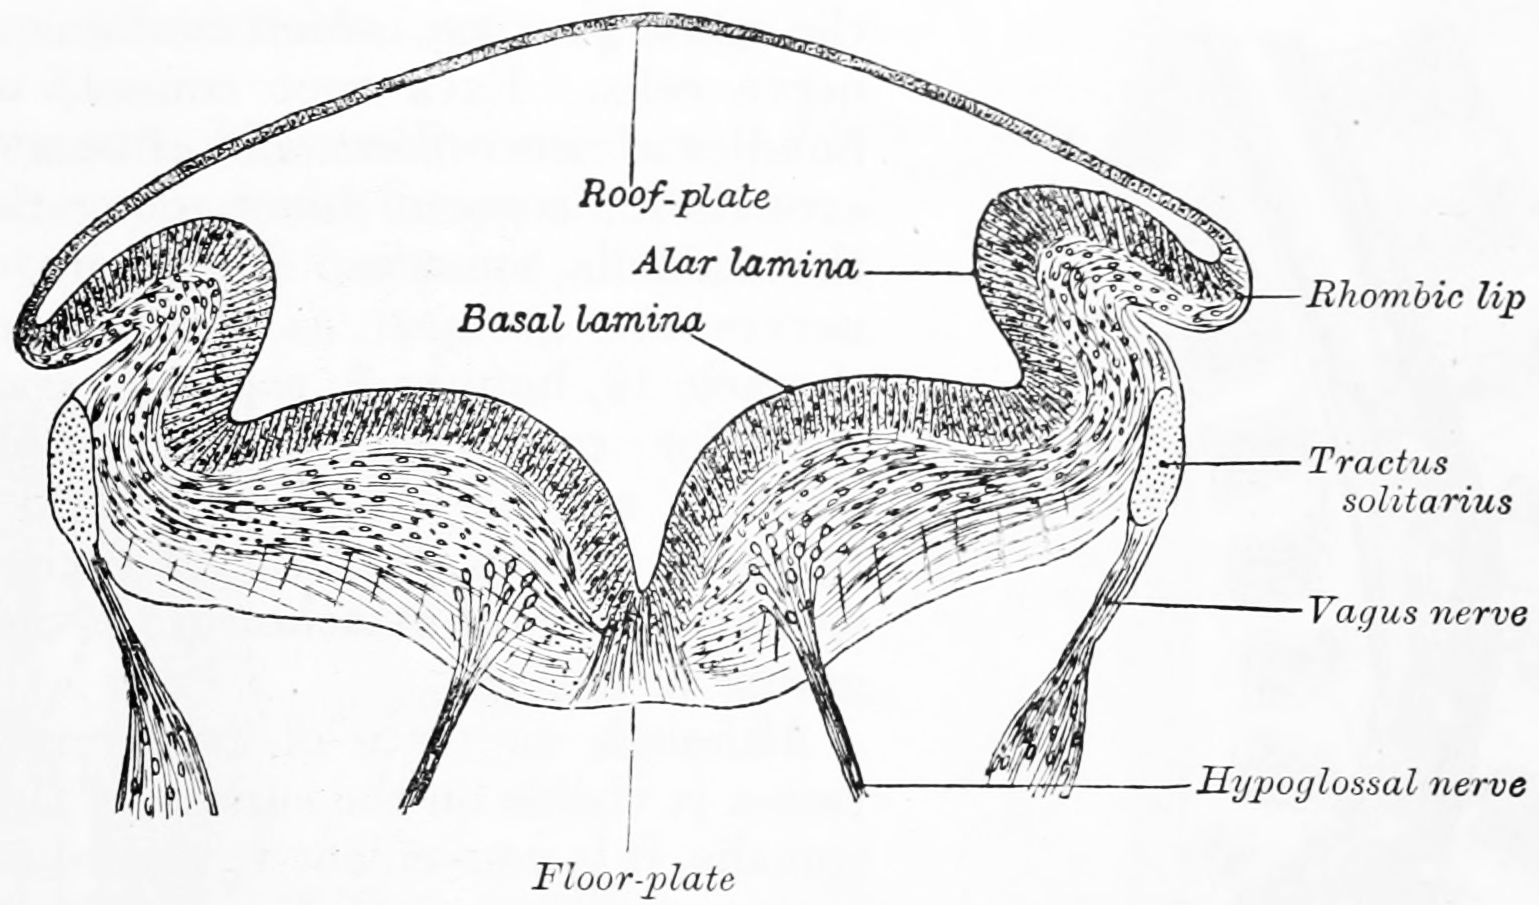
\includegraphics[width=0.7\linewidth]{./figures/development/GrayAnat1918p749} 

}

\caption{Transverse section of medulla oblongata of human embryo. From \href{https://archive.org/details/anatomyofhumanbo1918gray/page/n6/mode/2up}{Gray Henry, Anatomy of the Human Body. 20\textsuperscript{th} Edition, Lea \& Febiger, Philadelphia \& New York, 1918}}\label{fig:medullaoblongata}
\end{figure}

In the fifth week, the alar plate of the prosencephalon expands to form the cerebral hemispheres (the telencephalon). The basal plate becomes the diencephalon.



\begin{figure}

{\centering 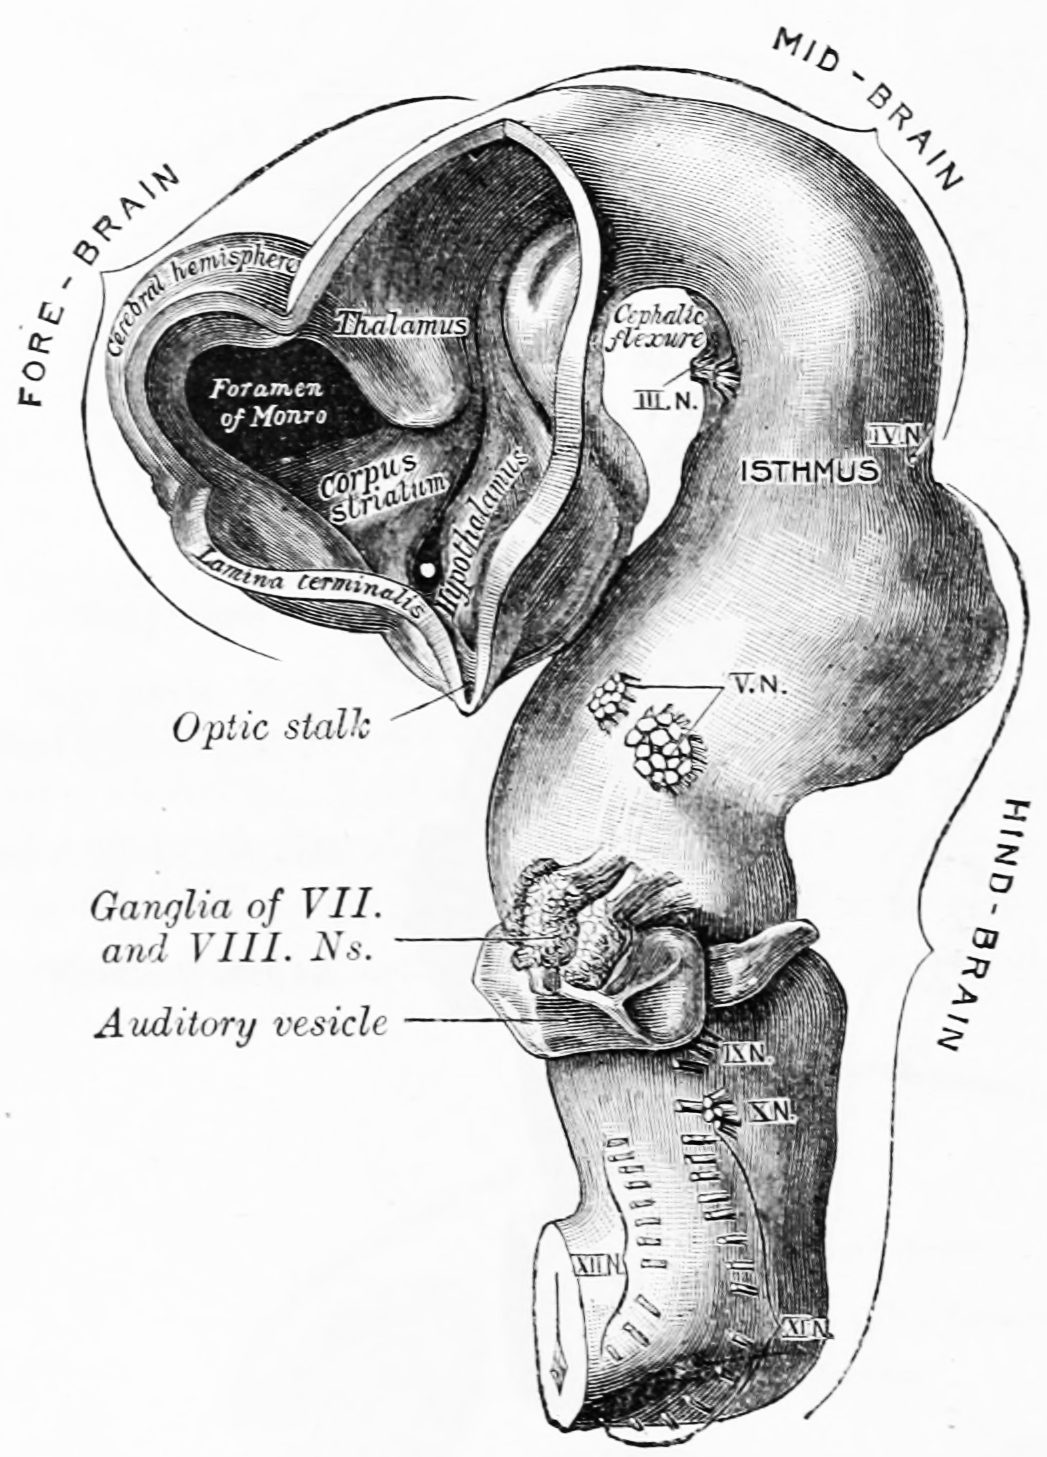
\includegraphics[width=0.7\linewidth]{./figures/development/GrayAnat1918p740} 

}

\caption{Brain of human embryo of four and a half weeks, showing interior of forebrain. From \href{https://archive.org/details/anatomyofhumanbo1918gray/page/n6/mode/2up}{Gray Henry, Anatomy of the Human Body. 20\textsuperscript{th} Edition, Lea \& Febiger, Philadelphia \& New York, 1918}}\label{fig:fourandahalf}
\end{figure}



\begin{figure}

{\centering 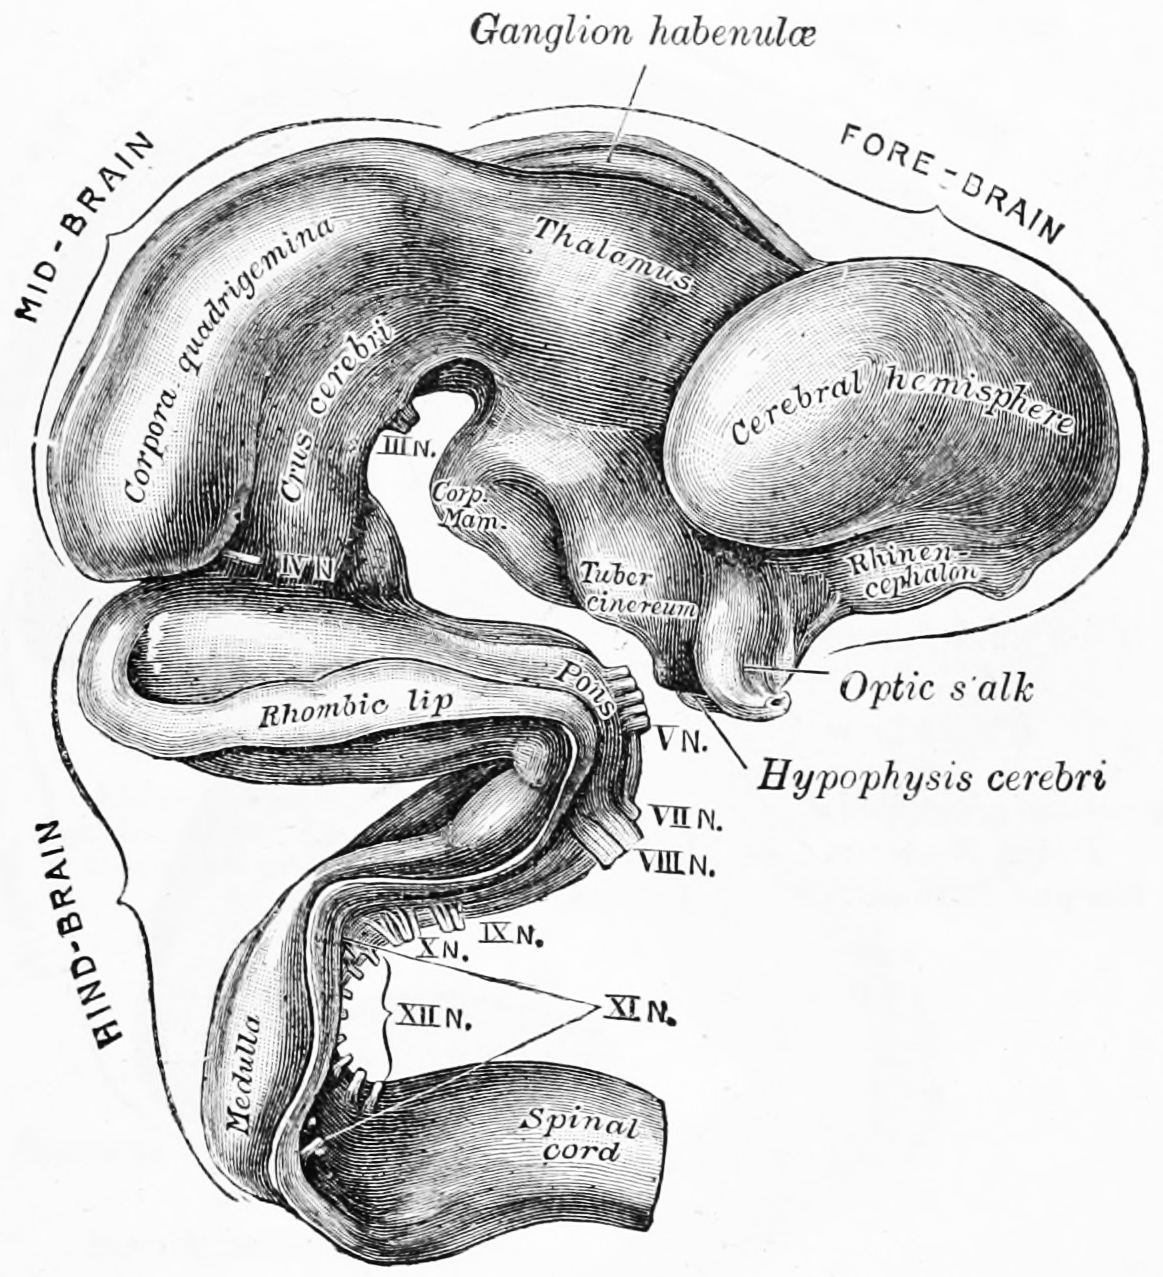
\includegraphics[width=0.7\linewidth]{./figures/development/GrayAnat1918p741} 

}

\caption{Exterior of brain of human embryo of five weeks. From \href{https://archive.org/details/anatomyofhumanbo1918gray/page/n6/mode/2up}{Gray Henry, Anatomy of the Human Body. 20\textsuperscript{th} Edition, Lea \& Febiger, Philadelphia \& New York, 1918}}\label{fig:fivexterior}
\end{figure}



\begin{figure}

{\centering 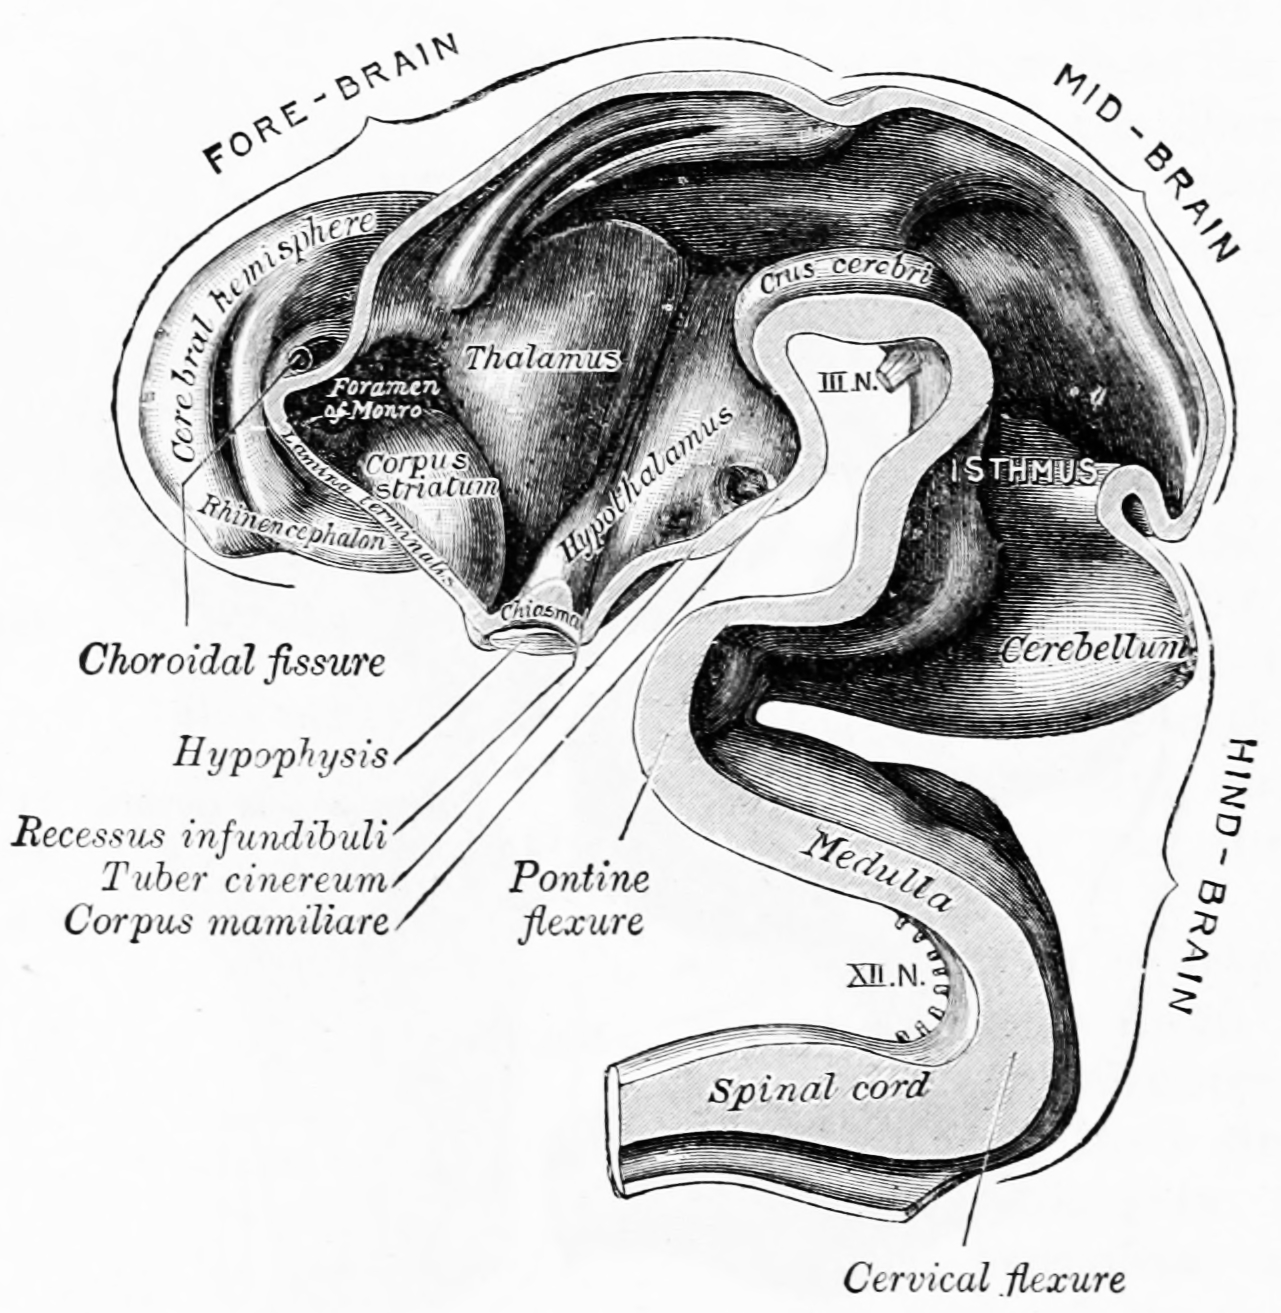
\includegraphics[width=0.7\linewidth]{./figures/development/GrayAnat1918p742} 

}

\caption{Interior of brain of human embryo of five weeks. From \href{https://archive.org/details/anatomyofhumanbo1918gray/page/n6/mode/2up}{Gray Henry, Anatomy of the Human Body. 20\textsuperscript{th} Edition, Lea \& Febiger, Philadelphia \& New York, 1918}}\label{fig:fiveinterior}
\end{figure}

The diencephalon, mesencephalon and rhombencephalon constitute the brain stem of the embryo. It continues to flex at the mesencephalon. The rhombencephalon folds posteriorly, which causes its alar plate to flare and form the fourth ventricle of the brain. The pons and the cerebellum form in the upper part of the rhombencephalon, whilst the medulla oblongata forms in the lower part.



\begin{figure}

{\centering 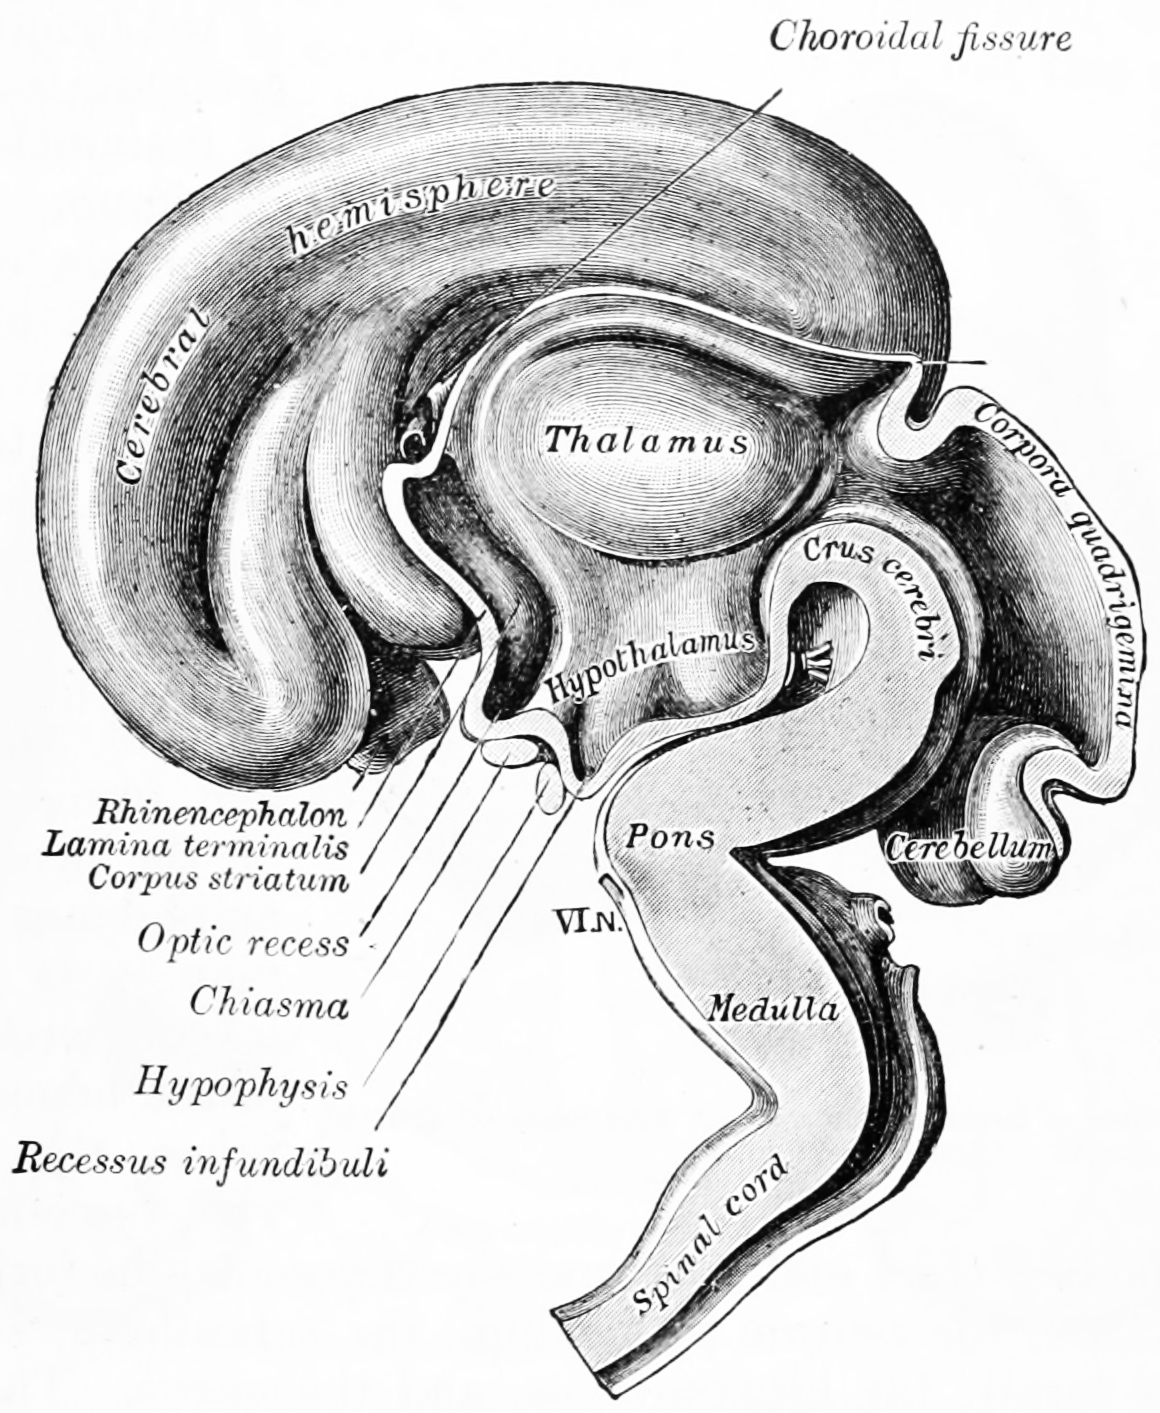
\includegraphics[width=0.7\linewidth]{./figures/development/GrayAnat1918p743} 

}

\caption{Interior of brain of human embryo of five weeks. From \href{https://archive.org/details/anatomyofhumanbo1918gray/page/n6/mode/2up}{Gray Henry, Anatomy of the Human Body. 20\textsuperscript{th} Edition, Lea \& Febiger, Philadelphia \& New York, 1918}}\label{fig:threemonths}
\end{figure}



\begin{figure}

{\centering 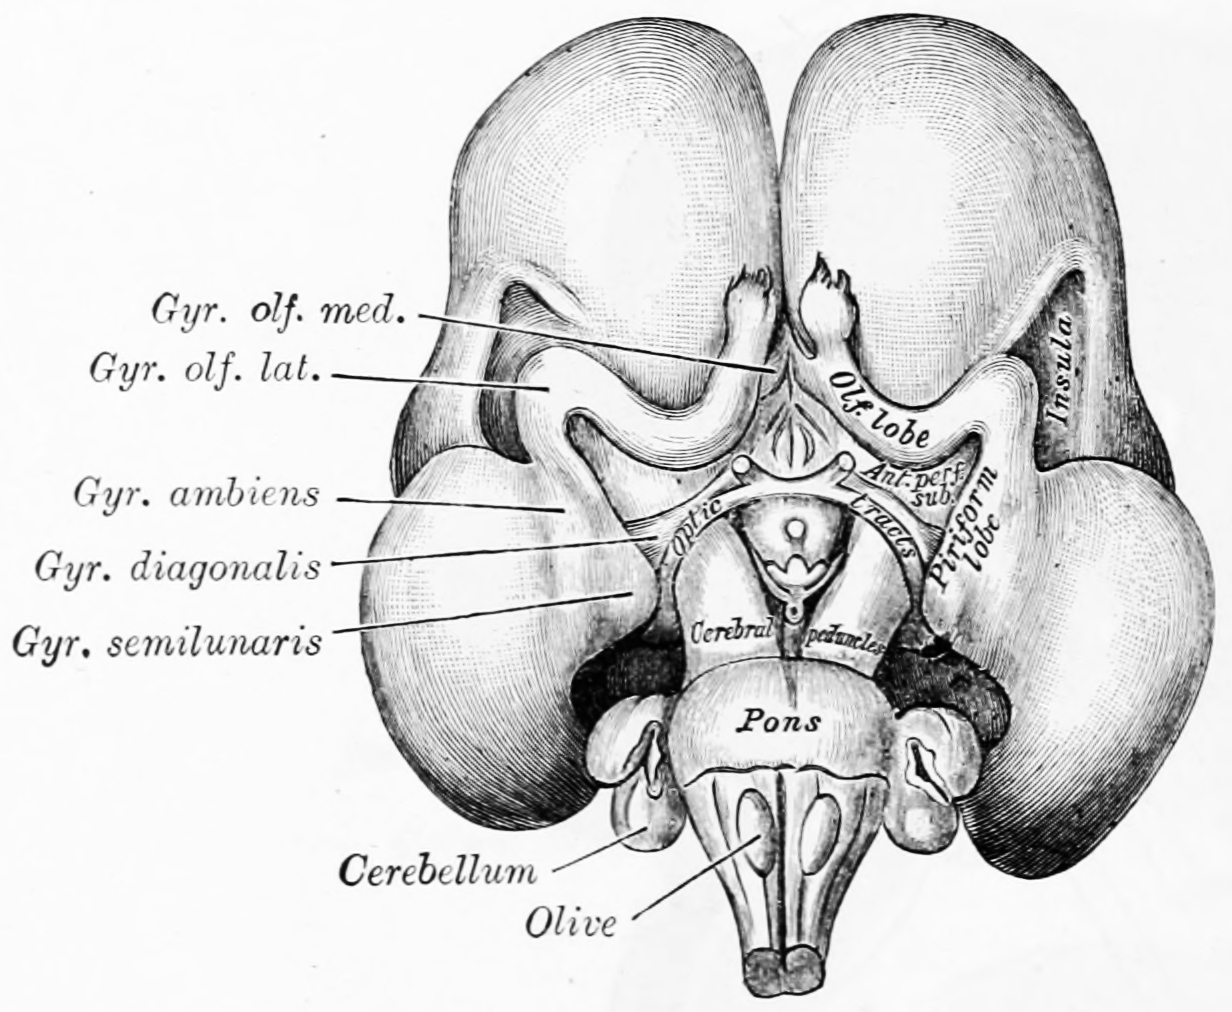
\includegraphics[width=0.7\linewidth]{./figures/development/GrayAnat1918p744} 

}

\caption{Inferior surface of brain of embryo at beginning of fourth month. From \href{https://archive.org/details/anatomyofhumanbo1918gray/page/n6/mode/2up}{Gray Henry, Anatomy of the Human Body. 20\textsuperscript{th} Edition, Lea \& Febiger, Philadelphia \& New York, 1918}}\label{fig:fourmonths}
\end{figure}



\begin{figure}

{\centering 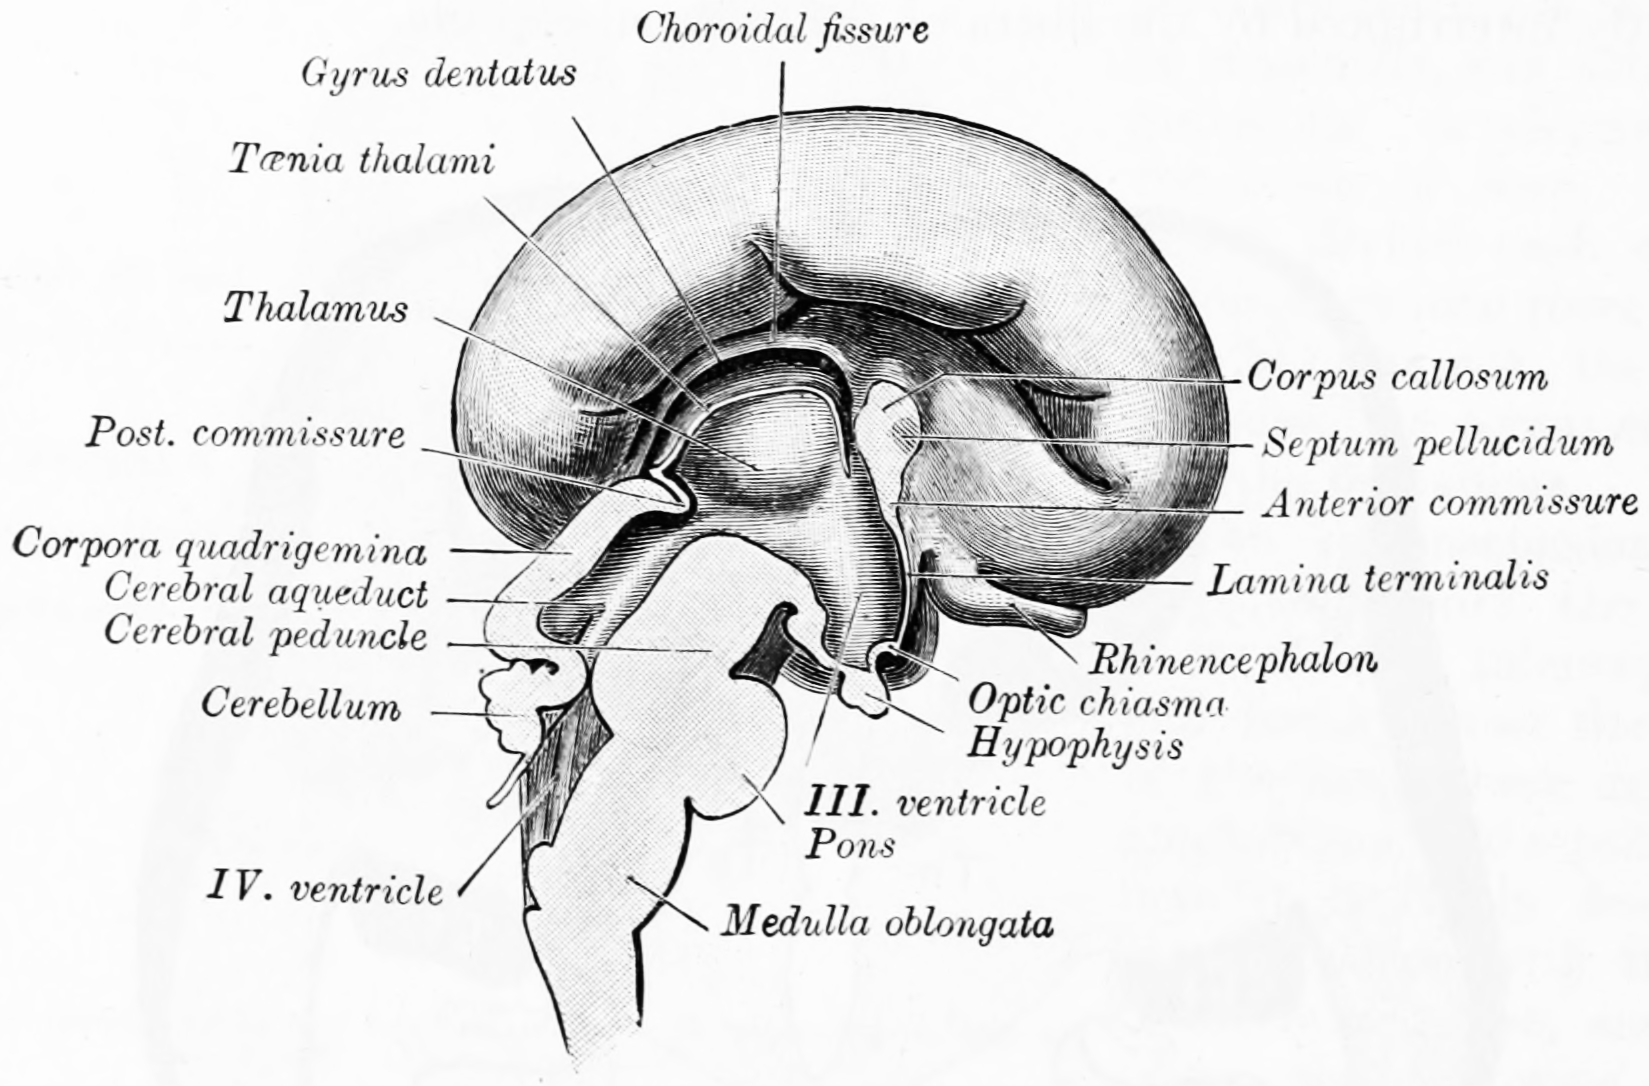
\includegraphics[width=0.7\linewidth]{./figures/development/GrayAnat1918p746} 

}

\caption{Median sagittal section of brain of human embryo of four months. From \href{https://archive.org/details/anatomyofhumanbo1918gray/page/n6/mode/2up}{Gray Henry, Anatomy of the Human Body. 20\textsuperscript{th} Edition, Lea \& Febiger, Philadelphia \& New York, 1918}}\label{fig:fourmonthsmedian}
\end{figure}

Some landmarks of neural development include the birth and differentiation of neurons from stem cell precursors, the migration of immature neurons from their birthplaces in the embryo to their final positions, outgrowth of axons and dendrites from neurons, guidance of the motile growth cone through the embryo towards postsynaptic partners, the generation of synapses between these axons and their postsynaptic partners, and finally the lifelong changes in synapses, which are thought to underlie learning and memory.



\begin{figure}

{\centering 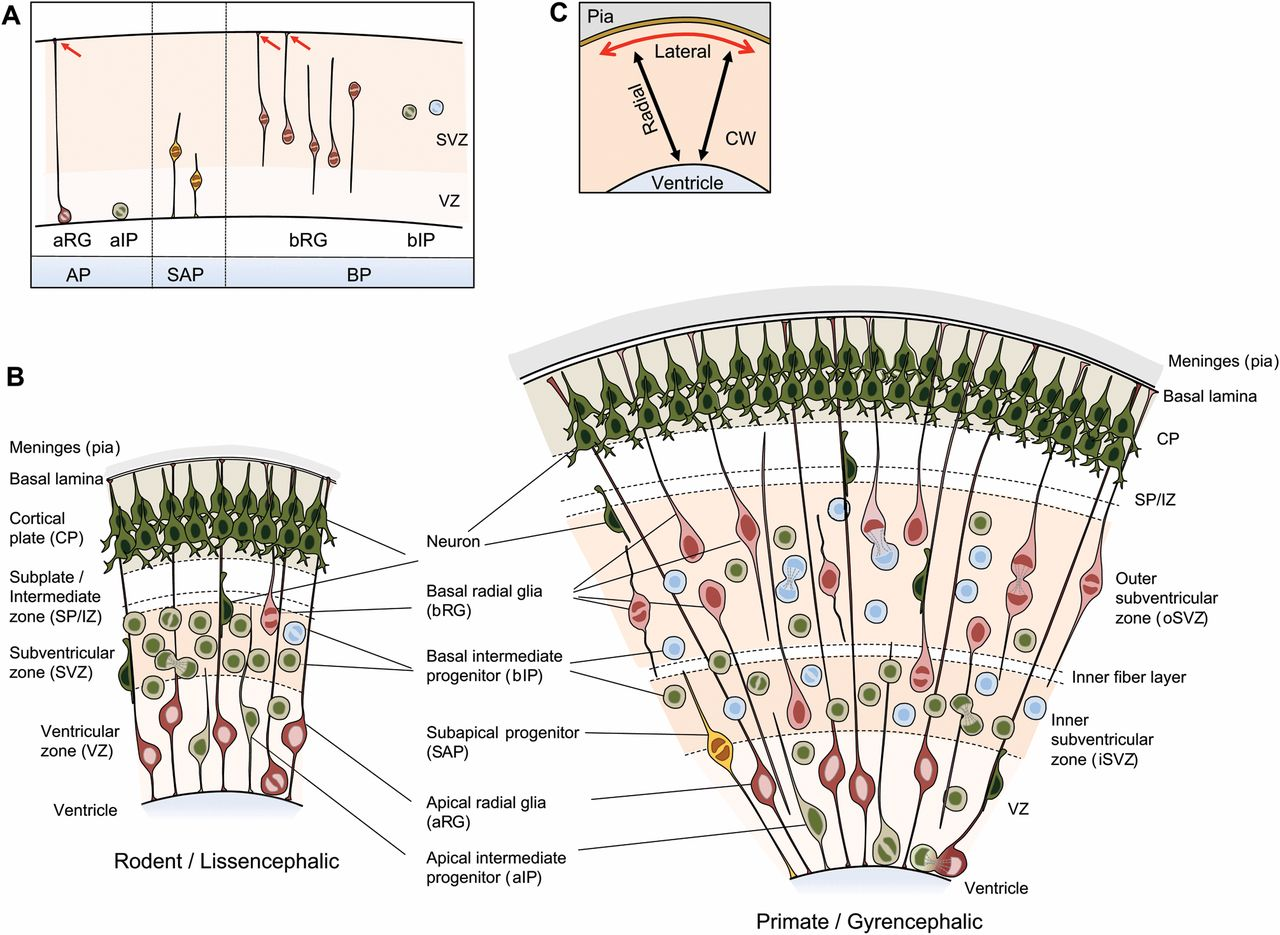
\includegraphics[width=0.7\linewidth]{./figures/development/neural_precursor} 

}

\caption{Neural precursor cell (NPC) types in the developing neocortex of representative lissencephalic and gyrencephalic species. (A) NPC types in the mammalian neocortex after the onset of neurogenesis, classified according to cell polarity, the presence of ventricular contact, and the location of mitosis. Red arrows indicate contact of the basal process with the basal lamina. Apical progenitors (APs), which include apical radial glia (aRG) and apical intermediate progenitors (aIPs), are defined by mitosis occurring at the ventricular surface and the presence of ventricular contact. Note that neuroepithelial cells (NECs), the primary APs that give rise to aRG and aIPs, are not depicted, as NECs prevail prior to the onset of neurogenesis. Subapical progenitors (SAPs) are defined by mitosis occurring at an abventricular location and the presence of ventricular contact. Basal progenitors (BPs), which comprise basal radial glia (bRG) and basal intermediate progenitors (bIPs), are defined by mitosis occurring at an abventricular location and the absence of ventricular contact. bRG subtypes (see Box 2 for more information) are also shown: proliferative bIP, blue; neurogenic bIP, green. (B) Coronal section of developing neocortex from a representative lissencephalic species, such as mouse or rat (left), and a representative gyrencephalic species, such as ferret or human (right), depicting the NPC types frequently observed in each of the germinal zones. (C) The major dimensions in which the developing neocortex is described: (1) radial (black arrows), i.e.~the ventricle-to-pia axis, corresponding to the apical-basal axis in terms of tissue polarity; and (2) lateral (red arrow), i.e.~the axis perpendicular to the radial axis. CW, cortical wall. From \href{https://dev.biologists.org/content/141/11/2182}{Marta Florio, Wieland B. Huttner(2014) Neural progenitors, neurogenesis and the evolution of the neocortex Development 2014 141: 2182-2194; doi: 10.1242/dev.090571}}\label{fig:neuralprecursor}
\end{figure}

Typically, these neurodevelopmental processes can be broadly divided into two classes: activity-independent mechanisms and activity-dependent mechanisms. Activity-independent mechanisms are generally believed to occur as hardwired processes determined by genetic programs played out within individual neurons. These include differentiation, migration and axon guidance to their initial target areas. These processes are thought of as being independent of neural activity and sensory experience. Once axons reach their target areas, activity-dependent mechanisms come into play. Although synapse formation is an activity-independent event, modification of synapses and synapse elimination requires neural activity.

Developmental neuroscience uses a variety of animal models including the mouse \emph{Mus musculus}, the fruit fly \emph{Drosophila melanogaster}, the zebrafish \emph{Danio rerio}, the frog Xenopus laevis, and the roundworm \emph{Caenorhabditis elegans}.

Myelination, formation of the lipid myelin bilayer around neuronal axons, is a process that is essential for normal brain function. The myelin sheath provides insulation for the nerve impulse when communicating between neural systems. Without it, the impulse would be disrupted and the signal would not reach its target, thus impairing normal functioning.

\hypertarget{patterning-of-the-nervous-system}{%
\section{Patterning Of The Nervous System}\label{patterning-of-the-nervous-system}}

In chordates, dorsal ectoderm forms all neural tissue and the nervous system. Patterning occurs due to specific environmental conditions - different concentrations of signaling molecules

The ventral half of the neural plate is controlled by the notochord, which acts as the `organiser'. The dorsal half is controlled by the ectoderm plate, which flanks either side of the neural plate.

Ectoderm follows a default pathway to become neural tissue. Evidence for this comes from single, cultured cells of ectoderm, which go on to form neural tissue. This is postulated to be because of a lack of BMPs, which are blocked by the organiser. The organiser may produce molecules such as follistatin, noggin and chordin that inhibit BMPs.

The ventral neural tube is patterned by sonic hedgehog (Shh) from the notochord, which acts as the inducing tissue. Notochord-derived Shh signals to the floor plate, and induces Shh expression in the floor plate. Floor plate-derived Shh subsequently signals to other cells in the neural tube, and is essential for proper specification of ventral neuron progenitor domains. Loss of Shh from the notochord and/or floor plate prevents proper specification of these progenitor domains. Shh binds Patched1, relieving Patched-mediated inhibition of Smoothened, leading to activation of the Gli family of transcription factors (GLI1, GLI2, and GLI3).

In this context Shh acts as a morphogen - it induces cell differentiation dependent on its concentration. At low concentrations it forms ventral interneurons, at higher concentrations it induces motor neuron development, and at highest concentrations it induces floor plate differentiation. Failure of Shh-modulated differentiation causes holoprosencephaly, a disorder in which the prosencephalon (the forebrain of the embryo) fails to develop into two hemispheres.

The dorsal neural tube is patterned by BMPs from the epidermal ectoderm flanking the neural plate. These induce sensory interneurons by activating Sr/Thr kinases and altering SMAD transcription factor levels.

Signals that control anteroposterior neural development include FGF and retinoic acid, which act in the hindbrain and spinal cord. The hindbrain, for example, is patterned by Hox genes, which are expressed in overlapping domains along the anteroposterior axis under the control of retinoic acid. The 3′ (3 prime end) genes in the Hox cluster are induced by retinoic acid in the hindbrain, whereas the 5′ (5 prime end) Hox genes are not induced by retinoic acid and are expressed more posteriorly in the spinal cord. Hoxb-1 is expressed in rhombomere 4 and gives rise to the facial nerve. Without this Hoxb-1 expression, a nerve similar to the trigeminal nerve arises.

\hypertarget{neurogenesis}{%
\section{Neurogenesis}\label{neurogenesis}}

Neurogenesis is the process by which neurons are generated from neural stem cells and progenitor cells. Neurons are `post-mitotic', meaning that they will never divide again for the lifetime of the organism.

Epigenetic modifications play a key role in regulating gene expression in differentiating neural stem cells and are critical for cell fate determination in the developing and adult mammalian brain. Epigenetic modifications include DNA cytosine methylation to form 5-methylcytosine and 5-methylcytosine demethylation. DNA cytosine methylation is catalyzed by DNA methyltransferases (DNMTs). Methylcytosine demethylation is catalyzed in several sequential steps by TET (\textbf{T}en-\textbf{e}leven \textbf{t}ranslocation methylcytosine dioxygenase) enzymes that carry out oxidative reactions (e.g.~5-methylcytosine to 5-hydroxymethylcytosine) and enzymes of the DNA base excision repair (BER) pathway.

\hypertarget{neuronal-migration}{%
\section{Neuronal Migration}\label{neuronal-migration}}

Neuronal precursor cells proliferate in the ventricular zone of the developing neocortex, where the principal neural stem cell is the radial glial cell. The first postmitotic cells must leave the stem cell niche and migrate outward to form the preplate, which is destined to become Cajal-Retzius cells and subplate neurons. These cells do so by somal translocation. Neurons migrating with this mode of locomotion are bipolar and attach the leading edge of the process to the pia. The soma is then transported to the pial surface by nucleokinesis, a process by which a microtubule ``cage'' around the nucleus elongates and contracts in association with the centrosome to guide the nucleus to its final destination. Radial glial cells, whose fibers serve as a scaffolding for migrating cells and a means of radial communication mediated by calcium dynamic activity, act as the main excitatory neuronal stem cell of the cerebral cortex or translocate to the cortical plate and differentiate either into astrocytes or neurons. Somal translocation can occur at any time during development.

Subsequent waves of neurons split the preplate by migrating along radial glial fibres to form the cortical plate. Each wave of migrating cells travel past their predecessors forming layers in an inside-out manner, meaning that the youngest neurons are the closest to the surface.

Most interneurons migrate tangentially through multiple modes of migration to reach their appropriate location in the cortex. An example of tangential migration is the movement of interneurons from the ganglionic eminence to the cerebral cortex. One example of ongoing tangential migration in a mature organism, observed in some animals, is the rostral migratory stream connecting subventricular zone and olfactory bulb.

Many neurons migrating along the anterior-posterior axis of the body use existing axon tracts to migrate along; this is called axophilic migration. An example of this mode of migration is in GnRH-expressing neurons, which make a long journey from their birthplace in the nose, through the forebrain, and into the hypothalamus. Many of the mechanisms of this migration have been worked out, starting with the extracellular guidance cues that trigger intracellular signaling. These intracellular signals, such as calcium signaling, lead to actin and microtubule cytoskeletal dynamics, which produce cellular forces that interact with the extracellular environment through cell adhesion proteins to cause the movement of these cells.

\hypertarget{neurotrophic-factors}{%
\section{Neurotrophic Factors}\label{neurotrophic-factors}}

The survival of neurons is regulated by survival factors, called trophic factors. The neurotrophic hypothesis was formulated by \href{https://en.wikipedia.org/wiki/Viktor_Hamburger}{Viktor Hamburger} and \href{https://en.wikipedia.org/wiki/Rita_Levi-Montalcini}{Rita Levi Montalcini} based on studies of the developing nervous system. Victor Hamburger discovered that implanting an extra limb in the developing chick led to an increase in the number of spinal motor neurons. Initially he thought that the extra limb was inducing proliferation of motor neurons, but he and his colleagues later showed that there was a great deal of motor neuron death during normal development, and the extra limb prevented this cell death. According to the neurotrophic hypothesis, growing axons compete for limiting amounts of target-derived trophic factors and axons that fail to receive sufficient trophic support die by apoptosis. It is now clear that factors produced by a number of sources contribute to neuronal survival.

\begin{itemize}
\tightlist
\item
  Nerve Growth Factor (NGF): Rita Levi Montalcini and \href{https://en.wikipedia.org/wiki/Stanley_Cohen_(biochemist)}{Stanley Cohen} purified the first trophic factor, Nerve Growth Factor, for which they received the Nobel Prize. There are three NGF-related trophic factors: BDNF, NT3, and NT4, which regulate survival of various neuronal populations. The Trk proteins act as receptors for NGF and related factors. Trk is a receptor tyrosine kinase. Trk dimerization and phosphorylation leads to activation of various intracellular signaling pathways including the MAP kinase, Akt, and PKC pathways.
\item
  CNTF: Ciliary neurotrophic factor is another protein that acts as a survival factor for motor neurons. CNTF acts via a receptor complex that includes CNTFRα, GP130, and LIFRβ. Activation of the receptor leads to phosphorylation and recruitment of the JAK kinase, which in turn phosphorylates LIFRβ. LIFRβ acts as a docking site for the STAT transcription factors. JAK kinase phosphorylates STAT proteins, which dissociate from the receptor and translocate to the nucleus to regulate gene expression.
\item
  GDNF: Glial derived neurotrophic factor is a member of the TGFb family of proteins, and is a potent trophic factor for striatal neurons. The functional receptor is a heterodimer, composed of type 1 and type 2 receptors. Activation of the type 1 receptor leads to phosphorylation of Smad proteins, which translocate to the nucleus to activate gene expression.
\end{itemize}

\hypertarget{activity-dependent-mechanisms-in-the-assembly-of-neural-circuits}{%
\section{Activity Dependent Mechanisms In The Assembly Of Neural Circuits}\label{activity-dependent-mechanisms-in-the-assembly-of-neural-circuits}}

The processes of neuronal migration, differentiation and axon guidance are generally believed to be activity-independent mechanisms and rely on hard-wired genetic programs in the neurons themselves. Research findings however have implicated a role for activity-dependent mechanisms in mediating some aspects of these processes such as the rate of neuronal migration, aspects of neuronal differentiation and axon pathfinding. Activity-dependent mechanisms influence neural circuit development and are crucial for laying out early connectivity maps and the continued refinement of synapses which occurs during development. There are two distinct types of neural activity we observe in developing circuits -early spontaneous activity and sensory-evoked activity. Spontaneous activity occurs early during neural circuit development even when sensory input is absent and is observed in many systems such as the developing visual system, auditory system, motor system, hippocampus, cerebellum and neocortex.

Experimental techniques such as direct electrophysiological recording, fluorescence imaging using calcium indicators and optogenetic techniques have shed light on the nature and function of these early bursts of activity. They have distinct spatial and temporal patterns during development and their ablation during development has been known to result in deficits in network refinement in the visual system. In the immature retina, waves of spontaneous action potentials arise from the retinal ganglion cells and sweep across the retinal surface in the first few postnatal weeks. These waves are mediated by neurotransmitter acetylcholine in the initial phase and later on by glutamate. They are thought to instruct the formation of two sensory maps- the retinotopic map and eye-specific segregation. Retinotopic map refinement occurs in downstream visual targets in the brain-the superior colliculus (SC) and dorsal lateral geniculate nucleus (LGN). Pharmacological disruption and mouse models lacking the β2 subunit of the nicotinic acetylcholine receptor has shown that the lack of spontaneous activity leads to marked defects in retinotopy and eye-specific segregation.

In the developing auditory system, developing cochlea generate bursts of activity which spreads across the inner hair cells and spiral ganglion neurons which relay auditory information to the brain. ATP release from supporting cells triggers action potentials in inner hair cells. In the auditory system, spontaneous activity is thought to be involved in tonotopic map formation by segregating cochlear neuron axons tuned to high and low frequencies. In the motor system, periodic bursts of spontaneous activity are driven by excitatory GABA and glutamate during the early stages and by acetylcholine and glutamate at later stages. In the cortex, early waves of activity have been observed in the cerebellum and cortical slices. Once sensory stimulus becomes available, final fine-tuning of sensory-coding maps and circuit refinement begins to rely more and more on sensory-evoked activity as demonstrated by classic experiments about the effects of sensory deprivation during critical periods.

\hypertarget{critical-periods}{%
\section{Critical Periods}\label{critical-periods}}

A critical period is a maturational stage in the lifespan of an organism during which the nervous system is especially sensitive to certain environmental stimuli. If, for some reason, the organism does not receive the appropriate stimulus during this ``critical period'' to learn a given skill or trait, it may be difficult, ultimately less successful, or even impossible, to develop certain associated functions later in life. Functions that are indispensable to an organism's survival, such as vision, are particularly likely to develop during critical periods. ``Critical period'' also relates to the ability to acquire one's first language. Researchers found that people who passed the ``critical period'' would not acquire their first language fluently.

For example, the critical period for the development of a human child's binocular vision is thought to be between three and eight months, with sensitivity to damage extending up to at least three years of age. Further critical periods have been identified for the development of hearing and the vestibular system.

Critical periods of plasticity occur in the prenatal brain and continue throughout childhood until adolescence and are very limited during adulthood. Two major factors influence the opening of critical periods: cellular events (i.e.~changes in molecular landscape) and sensory experience (i.e.~hearing sound, visual input, etc). Both need to coincide for the critical period to open properly. At the cellular level, critical periods are characterized by maturation of the inhibitory circuits. More precisely, factors such as brain-derived neurotrophic factor (BDNF) and orthodenticle homeobox 2 (Otx2) contribute to the maturation of a major class of inhibitory neurons: parvalbumin-positive interneurons (PV cells). Prior to the onset of the critical period, modulation of this circuit is hampered by early factors such as polysialic acid (PSA). PSA acts, in part, by preventing Otx2 interaction with PV cells. Soon after the opening of the critical period, PSA levels decrease, allowing PV cell maturation by activating inhibitory GABA\textsubscript{A} receptors that facilitate inhibitory circuit remodeling. Artificially removing PSA, or experimentally manipulating inhibitory transmission can result in early opening of the critical period. While the timing of these molecular events seems to be partially explained by clock genes, experience is crucial as sensory deprivation experiments have been shown to interfere with the proper timing of critical periods.

\hypertarget{activity-dependent-competition}{%
\subsection{Activity-dependent competition}\label{activity-dependent-competition}}

Hebbian theory guides the idea of activity-dependent competition: if two neurons both have the potential to make a connection with a cell, the neuron that fires more will make the connection.

This phenomenon of activity-dependent competition is especially seen in the formation of ocular dominance columns within the visual system. Early in development, most of the visual cortex is binocular, meaning it receives roughly equal input from both eyes. Normally, as development progresses, the visual cortex will segregate into monocular columns that receive input from only one eye. However, if one eye is patched, or otherwise prevented from receiving sensory input, the visual cortex will shift to favor representation of the uncovered eye. This demonstrates activity-dependent competition and Hebbian theory because inputs from the uncovered eye make and retain more connections than the patched eye.

Axon formation and growth is another key part of plasticity and activity-dependent competition. Axon growth and branching has been shown to be inhibited when the neurons electrical activity is suppressed below the level of an active neighbor. This shows that axonal growth dynamics are not independent but rather depend on the local circuits within which they are active (i.e.~the activity of the other neurons competing for connections).

Microglia inherently play a role in synaptic pruning during adolescence. As resident immune cells of the central nervous system, microglia's main role is phagocytosis and engulfment. Studies have found that during critical periods in the visual cortex, neural synapses become the target of microglial phagocytosis. Neurons who received less frequent input from retinal ganglion cells during early postnatal periods were more prone to be engulfed and pruned by microglia, as per monocular deprivation experiments. Similar results were found when manipulating G-coupled purinergic receptors on microglial processes. Blocking these receptors or performing a knockout experiment significantly lowered microglial interactions and synaptic pruning during the early visual cortex critical period. More recently, the expression of the complement component 4 gene has been found to significantly contribute to abnormally high levels of microglial synaptic pruning during early stages of development in schizophrenic neurons and microglia, suggesting a genomic connection between the immune system and critical periods.

Dendritic spine motility is the altering of the dendritic morphology of a neuron, specifically the appearing and disappearing of the small protrusions known as spines. In early postnatal development, spine motility has been found to be at very high levels. Due to its most pronounced occurrence during postnatal days 11 through 15, spine motility is thought to have a role in neurogenesis. Motility levels significantly decrease before the start of the visual cortex critical period and monocular deprivation experiments show that motility levels steadily decrease until the critical period is over, hinting that motility might not be explicitly involved in this process. However, binocular deprivation before eye-opening resulted in a significant up-regulation of spine motility until the peak of the critical period, resulting in controversial findings regarding the role of dendritic spine motility.

Another critical component of neuronal plasticity is the balance of excitatory and inhibitory inputs. Early in development, GABA, the major inhibitory neurotransmitter in the adult brain, exhibits an excitatory effect on its target neurons. However, due to changes in internal chloride levels due to the up-regulation of potassium chloride pumps, GABA then switches to inhibitory synaptic transmission. The maturation of the GABAergic inhibitory system helps to trigger the onset of critical periods. Strengthened GABAergic systems can induce an early critical period, while weaker GABAergic inputs can delay or even prevent plasticity. Inhibition also guides plasticity once the critical period has begun. For example, lateral inhibition is especially important in guiding columnar formation in the visual cortex. Hebbian theory provides insight on the importance of inhibition within neural networks: without inhibition, there would be more synchronous firing and therefore more connections, but with inhibition, fewer excitatory signals get through, allowing only the more salient connections to mature.

Critical period closure has been shown to be modulated by the maturation of inhibitory circuits, mediated by the formation of perineuronal nets around inhibitory neurons. Perineuronal nets (PNNs) are structures in the extracellular matrix formed by chondroitin sulfate proteoglycans, hyaluronan, and link proteins. These structures envelop the soma of inhibitory neurons in the central nervous system, appearing with age to stabilize mature circuits. PNN development coincides with the closure of critical periods, and both PNN formation and critical period timing is delayed in dark-rearing. For example, PNN digestion by ABC chondroitinase in rats leads to a shift in ocular dominance upon monocular deprivation, which is normally restricted to its critical period much earlier in development.

Additionally, PNNs are negatively charged, which is theorized to create a cation-rich environment around cells, potentially leading to an increased firing rate of inhibitory neurons, thereby allowing for increased inhibition after the formation of PNNs and helping to close the critical period. The role of PNNs in critical period closure is further supported by the finding that fast-spiking parvalbulmin-positive interneurons are often surrounded by PNNs.

Perineuronal nets have also been found to contain chemorepulsive factors, such as semaphorin3A, which restrict axon growth necessary for plasticity during critical periods. In all, these data suggest a role for PNNs in the maturation of CNS inhibition, the prevention of plastic axonal growth, and subsequently, critical period closure.

Another mechanism that closes the critical period is myelination. Myelin sheaths are formed by oligodendrocytes in the CNS that wrap around segments of axons to increase their firing speed. Myelin is formed in the early stages of development and progresses in waves, with brain areas of later phylogenetic development (i.e.~those associated with ``higher'' brain functions like the frontal lobes) having later myelination. The maturation of myelination in intracortical layers coincides with critical period closure in mice, which has led to further research on the role of myelination on critical period duration.

Myelin is known to bind many different axonal growth inhibitors that prevent plasticity seen in critical periods. The Nogo Receptor is expressed in myelin and binds to the axonal growth inhibitors Nogo and MAG (among others), preventing axon growth in mature, myelinated neurons. Instead of affecting the timing of the critical period, mutations of the Nogo receptor prolong the critical period temporarily. A mutation of the Nogo receptor in mice was found to extend the critical period for monocular dominance from around 20 -- 32 days to 45 or 120 days, suggesting a likely role of the myelin Nogo receptor in critical period closure.

Additionally, the effects of myelination are temporally limited, since myelination itself may have its own critical period and timing. Research has shown that social isolation of mice leads to reduced myelin thickness and poor working memory, but only during a juvenile critical period. In primates, isolation is correlated with abnormal changes in white matter potentially due to decreased myelination.

In all, myelin and its associated receptors bind several important axonal growth inhibitors which help close the critical period. The timing of this myelination, however, is dependent on the brain region and external factors such as the social environment.

While the presence or absence of sensory experiences most robustly shapes brain development during the critical period, the behavioral context (i.e.~the amount of attention, arousal, fear and reward experienced) concurrent with the sensory inputs have been suggested to be important in regulating the brain remodeling mechanisms. In terms of brain connectivity, these behavioral and contextual inputs activate the neuromodulatory system, which have substantial connectivity to the cortex The molecular effectors released by the neuromodulatory system are called neuromodulators, which include acetylcholine, dopamine, and noradrenaline among others. Investigating the effect of these molecules, as well as the neurons that release and bind them, has been one approach to elucidate the biology of neuromodulation. Research using this approach has highlighted the role of neuromodulation in sensory processing during the critical period. For example, on the one hand, in kittens, a shift in ocular dominance resulting from monocular deprivation during the critical period is reduced by combined destruction of noradrenergic and cholinergic neurons. In addition, prenatal exposure to selective serotonin reuptake inhibitors (SSRI) causes a shift in perceptual narrowing on language to earlier in development. On the other hand, neuromodulatory stimulation has been shown to induce brain plasticity in adult mice. While being subjected to cholinergic or dopaminergic stimulation, adult mice listening to a tone of specific frequency exhibited expansion of the tonotopic area in the auditory cortex that responds specifically to sounds of that frequency.

Mechanistically, neuromodulation is increasingly being recognized for its fine-tuning of the PV cell-mediated inhibition of excitatory pyramidal neurons' soma. Central to the neuromodulatory regulation of PV cell activity is the existence of distinct subsets of inhibitory neurons, which are responsive to activation by neuromodulators and which inhibit PV cells. Within these cells, some also inhibit specific pyramidal cell dendrites. By inhibiting PV cells activity, the neuromodulator-sensitive inhibitory cells such as those expressing Vasoactive intestinal peptide (VIP) or somatostatin (SST) lift the inhibition of the pyramidal neurons; in other words, the activity of VIP and SST-expressing cells result in the disinhibition of pyramidal neurons. Then, by inhibiting only certain dendritic branches of these now dis-inhibited pyramidal neurons, the neuromodulation-activated cells allow select sensory inputs to excite the pyramidal neurons and be represented in the brain circuitry. Thus, in a landscape of global inhibition by maturing inhibitory signaling, neuromodulation allows windows of dis-inhibition, temporally and spatially, that allow behaviorally important sensory inputs the opportunity to influence the brain.

In mammals, neurons in the brain that process vision actually develop after birth based on signals from the eyes. A landmark experiment by David H. Hubel and Torsten Wiesel (1963) showed that cats that had one eye sewn shut from birth to three months of age (monocular deprivation) only fully developed vision in the open eye. They showed that columns in the primary visual cortex receiving inputs from the other eye took over the areas that would normally receive input from the deprived eye. In general electrophysiological analyses of axons and neurons in the lateral geniculate nucleus showed that the visual receptive field properties was comparable to adult cats. However, the layers of cortex that were deprived had less activity and fewer responses were isolated. The kittens had abnormally small ocular dominance columns (part of the brain that processes sight) connected to the closed eye, and abnormally large, wide columns connected to the open eye. Because the critical period time had elapsed, it would be impossible for the kittens to alter and develop vision in the closed eye. This did not happen to adult cats even when one eye was sewn shut for a year because they had fully developed their vision during their critical period. Later experiments in monkeys found similar results consistent with the strong critical period.

In a follow-up experiment, Hubel and Wiesel (1963) explored the cortical responses present in kittens after binocular deprivation; they found it difficult to find any active cells in the cortex, and the responses they did get were either slow-moving or fast-fatiguing. Furthermore, the cells that did respond selected for edges and bars with distinct orientation preferences. Nevertheless, these kittens developed normal binocularity. Hubel and Wiesel first explained the mechanism, known as orientation selectivity, in the mammalian visual cortex. Orientation tuning, a model that originated with their model, is a concept in which receptive fields of neurons in the LGN excite a cortical simple cell and are arranged in rows. This model was important because it was able to describe a strong critical period for the proper development of normal ocular dominance columns in the lateral geniculate nucleus, and thus able to explain the effects of monocular deprivation during this critical period. The critical period for cats is about three months and for monkeys, about six months.

In a similar experiment, Antonini and Stryker (1993) examined the anatomical changes that can be observed after monocular deprivation. They compared geniculocortical axonal arbors in monocularly deprived animals in the long term (4- weeks) to short term (6--7 days) during the critical period established by Hubel and Wiesel (1993). They found that in the long term, monocular deprivation causes reduced branching at the end of neurons, while the amount of afferents allocated to the nondeprived eye increased. Even in the short term, Antonini and Stryker (1993) found that geniculocortical neurons were similarly affected. This supports the aforementioned concept of a critical period for proper neural development for vision in the cortex.

Studies of people whose sight has been restored after a long blindness (whether from birth or a later point in life) reveal that they cannot necessarily recognize objects and faces (as opposed to color, motion, and simple geometric shapes). Some hypothesize that being blind during childhood prevents some part of the visual system necessary for these higher-level tasks from developing properly. The general belief that a critical period lasts until age 5 or 6 was challenged by a 2007 study that found that older patients could improve these abilities with years of exposure.

Expression of the protein Lynx1 has been associated with the normal end of the critical period for synaptic plasticity in the visual system.

\hypertarget{brain-plasticity}{%
\section{Brain plasticity}\label{brain-plasticity}}

Neuroplasticity, also known as brain plasticity, or neural plasticity, is the ability of the brain to change continuously throughout an individual's life, e.g., brain activity associated with a given function can be transferred to a different location, the proportion of grey matter can change and synapses may strengthen or weaken over time. The aim of neuroplasticity is to optimize the neural networks during phylogenesis, ontogeny and physiological learning, as well as after a brain injury. Research in the latter half of the 20th century showed that many aspects of the brain can be altered (or are ``plastic'') even through adulthood. However, the developing brain exhibits a higher degree of plasticity than the adult brain.

Activity-dependent plasticity is a form of functional and structural neuroplasticity that arises from the use of cognitive functions and personal experience; hence, it is the biological basis for learning and the formation of new memories. Activity-dependent plasticity is a form of neuroplasticity that arises from intrinsic or endogenous activity, as opposed to forms of neuroplasticity that arise from extrinsic or exogenous factors, such as electrical brain stimulation- or drug-induced neuroplasticity. The brain's ability to remodel itself forms the basis of the brain's capacity to retain memories, improve motor function, and enhance comprehension and speech amongst other things. It is this trait to retain and form memories that is associated with neural plasticity and therefore many of the functions individuals perform on a daily basis. This plasticity occurs as a result of changes in gene expression which are triggered by signaling cascades that are activated by various signaling molecules (e.g., calcium, dopamine, and glutamate, among many others) during increased neuronal activity.

The brain's ability to adapt toward active functions allows humans to specialize in specific processes based on relative use and activity. For example, a right-handed person may perform any movement poorly with his/her left hand but continuous practice with the less dominant hand can cause one to become ambidextrous. Another example is if someone was born with a neurological disorder such as major depressive disorder or had a stroke that resulted in a disorder, then they are capable of retrieving much of their lost function through practice, which in turn ``rewires'' the brain to mitigate neurological dysfunction.
Neuroplasticity can be observed at multiple scales, from microscopic changes in individual neurons to larger-scale changes such as cortical remapping in response to injury. Behavior, environmental stimuli, thought, and emotions may also cause neuroplastic change through activity-dependent plasticity, which has significant implications for healthy development, learning, memory, and recovery from brain damage. At the single cell level, synaptic plasticity refers to changes in the connections between neurons, where as non-synaptic plasticity refers to changes in their intrinsic excitability.

Activity-dependent plasticity plays a very important role in learning and in the ability of understanding new things. It is responsible for helping to adapt an individual's brain according to the relative amount of usage and functioning. In essence, it is the brain's ability to retain and develop memories based on activity-driven changes of synaptic strength that allow stronger learning of information. It is thought to be the growing and adapting quality of dendritic spines that provide the basis for synaptic plasticity connected to learning and memory. Dendritic spines accomplish this by transforming synaptic input into neuronal output and also by helping to define the relationship between synapses.


